\setcounter{page}{1} \pagenumbering{arabic}
\chapter{Introduction} 

This monograph presents theoretical and empirical considerations in the field of entrepreneurship. The fundamental idea is that the act of entrepreneurship expresses a crucial development of the social division of labour; a phenomenon addressed during the 18th century. We specifically recall the work of Adam~\cite{Smith1776} who, in his discussion on the generation of economic wealth, places the operation and evolution of the division of labour at the forefront. Although Smith focusses on the economic activities of society from a dynamic point of view, his concept of the \emph{invisible hand}---and the theory that an economy is normally in some naturally \emph{stable state}---has dominated theoretical discourse. Over the last two centuries the dynamic concept of economic interaction that Smith sought to discuss in the \emph{Wealth of Nations} has been substituted for a more static analysis, and the importance that he placed on increasing returns to specialisation and the operation of the division of labour has been diluted. This is reflected in general equilibrium analysis, a cornerstone of traditional economic theory.

The arrival of an economic system to a well-defined steady state, as expressed in general equilibrium modelling, contradicts the notion of active entrepreneurship. Entrepreneurship is a dynamic force that cannot emerge from a static economic steady state as defined by general equilibrium theory. This is a perspective that is shared with more heterodox economic writers such as~\citet{Schumpeter1942}. As a consequence, the notion of the entrepreneur and the act of entrepreneurship lacks definition and application in traditional economic theory. The most compelling definitions of entrepreneurship emerge within more heterodox strands of economics and sociology, which subsequently lack an elaborate theoretical basis. The outcome is a shallow insight into the environmental context of entrepreneurship and the result that entrepreneurship has on the organisation and distribution of power within society.

The theory developed in this monograph expresses the importance of institutional structures and the organisation of trade to the process of entrepreneurship. We value the general equilibrium concept as an expression of a specific and efficient form of organisation of the trade processes in the economy. The assumptions enforced by the Walrasian model lead to the formation of a market whereby the axiom of perfectly competitive behaviour is expressed. The resulting organisation of society is perfectly formed, thus allowing no role for entrepreneurial actions: as a result, the institutional structure is rigid. A more general way to consider the organisation of trade processes is through the perspective of a network; an interaction structure that emerges as a consequence of a pattern of exchanges between a population of agents under a given institutional system of governance and mechanism of trade. Under the Walrasian model of general equilibrium, a complete network emerges representing perfectly efficient market processes. In reality, networked markets are imperfectly connected; structural holes and opportunities for brokerage exist. These structural imperfections provide opportunities for entrepreneurial actors to exploit.

Throughout this monograph we propose other forms of organisation and trade processes in the economy, such as markets with imperfect structure, costly interactions, and heterogeneous positions of economic agents that derive from specialisation and the social division of labour. We establish a fundamentally dynamic theory of the economy, thus allowing for the development of entrepreneurship in a natural way. This is the purpose of our initial theorising; it regards how we perceive the interaction space of the economy and allows us to appropriately define the entrepreneur and act of entrepreneurship. From this, we can analyse entrepreneurial action and power within the context of empirical examples. Overall, we feel that this provides a better description of how real-world economic processes take place.

The monograph is divided into three Parts; each of which discusses certain modelling aspects of the economy under different forms of trade organisation, socio-economic states and entrepreneurial activities. In this introductory chapter we propose the aim of the monograph and provide an overview of key concepts discussed throughout; including the social division of labour and both social and economic networks. In doing so we also provide our perception of conventional economic modelling techniques, particularly under the Arrow-Debreu model, and the notion of a socially structured economy.

\section{Aim and motivation}
\label{sec:aimMotivation}

Traditional economic theory is founded on the basis of \emph{methodological individualism}, \emph{methodological instrumentalism} and \emph{equilibration}. With methodological individualism, the individual decision-making agent has a central position in the theory. In most cases, an economy is described as a configuration of such individual economic agents, each of which attempts to optimise some well-defined pre-determined goal or objective. In this configuration it is assumed that the economic agent possesses the tools to optimise their utility; this is the crux of methodological instrumentalism \citep{Arnsperger2006}. This implies that economic decision processes in the economy are determined by the individual decision behaviour of these economic agents and by the configuration in which these economic agents are located. The outcome of this interaction is an equilibrium state represented as an organisational steady state. The economic system transitions from one steady state to another through some exogenous shock; suggesting that any dynamism is purely transitory and is fundamentally ill-defined---a \emph{manna from heaven}.

An additional assumption is that the individual economic agent can be described entirely with the use of individual attributes only. Examples of these individual attributes are an endowment bundle of commodities, individual production capacities and an individual preference relation on the set of well-defined, achievable commodity bundles for the particular economic agent. An illustration of this reliance on methodological individualism is with respect to the traditional Arrow-Debreu model of a perfectly competitive market system. This model contains a population of individual economic agents partitioned into a set of consumers and a set of producers. Consumers attempt to optimise a certain individual preference relation over the collection of achievable commodity bundles, while producers try to maximise their profit given their individual production capacities. These economic agents are placed within the context of a system of perfectly competitive markets, which puts certain constraints on the abilities of agents. The major constraint is given by the price levels determined by the market. Consumers limit themselves in terms of budget sets while producers adapt their production plan to maximise their profits. There is no consideration for other socially constructed characteristics that have an influence on the preferences and abilities of the individual decision-maker: the price level is the only `social' aspect that has a considerable influence on the population of individuals.

Within this context, the application of methodological individualism is very specific. Only individual decision-makers are participating in the processes that take place within the economy. Its use suggests that economic agents are essentially individuals who are interacting with each other according to the exogenous rules of the economic organisation and not with each other as a primitive social characteristic in their behaviour. This illustrates that the traditional method of microeconomic theorising implicitly involves a certain requirement on the `rules of the game'.

\medskip \noindent In this monograph, we recognise that the rules of the game---which are reflected in the social and economic structure of the economy---are crucial in the design of a descriptive model of social and economic processes in that economy. Indeed, all economies are \emph{socially structured}; they are characterised by the socially constructed institutions and systems of governance that in turn guide the actions of a population of interconnected and interdependent agents.

We stress that social structure within this framework is flexible and, as such, is enforced and manipulated by economic agents themselves. This suggests that economic agents are not just individual decision-makers, but are decision-makers within a certain organisational environment consisting of a social and economic interaction architecture and behaviouristic conventions. An economic agent is still considered to be a decision-maker with some individual objective goal, but is also explicitly considered within some organisational environment informed by a well-defined governance system. The fact that an agent is considered as embedded within an organisational environment, leads to the acceptance of certain so-called \emph{social constraints} on the behaviour of that economic agent. Specifically, the agent's activity is contained within a matrix of interactions thus suggesting that the structure of interactions can also impose a constraint to their decision-making. We claim that constraints for some agents provide opportunities for others; distinctively, imperfections within society can provide opportunities for entrepreneurial activity.

Arguably, the Arrow-Debreu model expresses a socially structured economy; albeit in a limited sense. The interactions of a finite set of purely individualistic decision-makers generate an idealistic market characterised by an objective price level for the exchange of a good. The social and economic structure developed is limited in the sense that it results in a static market mechanism shorn of all other social influences. In the real world, prices are not objective as in Arrow-Debreu style general equilibrium modelling. The notion of perfect competition is purely \emph{idealised}. Market imperfections, bounded human rationality, institutional structures and incomplete network architectures explain disparity and subjectivity in price levels. \citet{Blume2009} provide a model of exchange on a network based on the notion of Nash equilibrium. The model suggests that agents possessing dominant positions within a network of relations can influence price levels exposed to both producers and consumers. Institutions and socially constructed customs and cultures inform preferences and thus price levels within markets. We embrace these fundamentally social aspects of the economy within our modelling.

\subsection{Objectives}

The aim of the monograph is to provide a theory of entrepreneurship and the entrepreneurial function within socially structured economies. Our first objective in achieving this is to develop a perspective of embedded economic activity based on a population of specialised economic agents that form a functional social division of labour. The deepening of the social division of labour leads to a generation of wealth that benefits society as a whole. Specifically, we take a \emph{relational perspective} in which to view the foundations of social and economic phenomena. This foundation, established in Chapter~\ref{ch:relationalperspective}, provides a theory of social and economic interaction based on the use of socially embedded systems of governance which are successfully utilised given a foundation of trust. The relational perspective developed embraces Smith, yet deviates substantially from the traditional paradigm of the economics discipline founded on the Arrow-Debreu model.

The second objective is to explain and illustrate the role of the entrepreneur within the relational perspective and highlight the impact that entrepreneurship has on the evolution of the social division of labour, and therefore the development or, in some instances, the regression of the economy. Within our theory we note that the entrepreneur can have an impact on different dimensions of the economy: specifically impacting economic agents themselves, the economic interaction networks, and the institutions of the interaction environment.

The third objective is to provide a distinction between the act of entrepreneurship and the entrepreneurial function of the economy. The latter relates to the adaptive and creative act that many economic agents perform in producing outputs; this facilitates differentiation and great economic wealth, but not necessarily a new species of work or profession. The former relates to incredibly creative and disruptive acts that are reflective in the organisation of society and the interaction of new specialisations.

The final objective is to complement our theoretical discussion of the relational perspective and entrepreneurship with empirical analyses of entrepreneurial activities. This involves creating a set of tools that allows us to analyse data in a pragmatic way. From these tools, we can identify influential positions and activities within a networked economy. Our two main empirical applications are relate to the network of elite Florentine families and the directorate network of New York City during the beginning on the 20th century.

\medskip\noindent In developing a relational perspective of social and economic---otherwise denoted as~\emph{socio-economic}---activity we first provide a detailed insight into our central unit of analysis: the human agent. We investigate the micro-foundational elements of the human agent; elaborating on the agents' innate ability to form social relationships. We stress the co-evolution of the human brain with the growth of the increasingly complex social environment that it must navigate and organise. In doing so, we align our analysis with the hypothesis that the human brain has not developed in order to understand informational attributes of our environment but, converse to the conventional wisdom, our brains still remain imperfect in understanding environmental information. The economic decisions we make in complex situations are only made on the basis of bounded rationality, with informational constraints, and in situations of uncertainty.

Our characterisation of the economic agent relaxes two important assumptions of traditional economic modelling. The first is that there exists a dichotomy between consumers and producers: the population of economic agents is partitioned into two non-intersecting sets, each of which interact between, but not within, one another. The second refers to the structure of production possibilities, which do not lend themselves to Smith's notion of increasing returns to specialisation. As a consequence, specialised producers do not emerge naturally within the Walrasian framework. In modelling economic agents, we allow for increasing returns to specialisation through learning, which stands in contrast to the Arrow-Debreu model and other general equilibrium models developed from its foundation.

From this perspective of the human actor, and the society in which she is embedded, we elaborate on a theory that takes a topological analysis of social and economic interactions through the evolution of institutions that facilitate exchange and the deepening of the division of labour. We suggest that the division of labour naturally leads to the formation of relational networks, and from this we investigate the evolution of these relational networks---and thus the evolution of the economy---through the perspective of the entrepreneurial function, which primarily acts to extend the division of labour. As such we contend that the evolution of the socio-economic networks, and the systems of governance that hold them together, can only be explained through the use of the entrepreneurial function and the subsequent extension, or contraction, of the social division of labour.

\subsection{Motivation}

The development of a novel model for investigating socio-economic phenomena has come from two overlapping concerns. The first is prompted by the apparent deficiency in mainstream theory to convincingly address the emergence of new organisational structures and technologies and to fully incorporate the entrepreneurial function within the economy. The entrepreneur is left undeveloped in many formal economic theories. A deficiency of mainstream theories lies in appropriately modelling the entrepreneurial function. The nature of this deficiency derives from the use of Walrasian axioms based on the notion of general equilibrium, as expressed above. Economic markets tend to converge to a predetermined equilibrium state within which unique market-clearing prices for homogeneous outputs emerge. At such a point it is difficult to endogenously integrate the development of an innovative technology into the model without having to assume its eventual existence which exogenously disrupts the growth of the economy. Well-established endogenous growth models have been created to formally explain how the generation of ideas from a research sector can lead to economic growth~\citep{Romer1990}, however, these models do not truly integrate differentiated and innovative commodities, nor do they convincingly integrate the entrepreneur and innovative entrepreneurial actions. In order to integrate the entrepreneurial function, it may be beneficial to maintain that the notion of static equilibrium as a purely intellectual concept. Much like the Austrian perspective on the matter, opportunities arise when the economy is imperfect and out of equilibrium; and, much like the Schumpeterian perspective, the entrepreneur's actions actively \emph{disequilibriate} the economy thus facilitating the emergence of increasingly more opportunities and innovation to take place meaning that equilibrium will never emerge. Thus, we should advocate that the economy has the potential to be in a continual state of dynamism.

Second, and perhaps more importantly, there seems to be an underlying disgruntlement within the economics discipline which has especially come to light in both academic and popular literature since the global financial crisis of 2008. Some economists believe that the fundamental problem derives from the fact that the economics discipline has become progressively divorced from economic reality.~\citet{Hodgson2009},~\citet{Smith2010} and~\citet{Keen2011} have appealed for a complete reform of the economics discipline as opposed to continually building increasingly esoteric and irrelevant mathematical models on top of a broken paradigm. These critics agree that the focus of the discipline has to change from its overwhelming focus on elegant general equilibrium models to a more pragmatic and empirically founded approach. Where the discipline should concentrate its efforts remains debatable and highly sensitive to the opinion of the specific economist. We agree with Hodgson that, in order to be pragmatic, we must orient ourselves to understanding real-world institutional environments and actors. However, it is important to initially be more fundamental than that; we must first understand the mechanisms concerning the embeddedness of economic activity in social constructs, the implications of the resulting division of labour and trade, and the development of innovation which is at the heart of the entrepreneurial function.

This disgruntlement concerning the state of the economics discipline is far from new. Nobel prize winners, such as Wassily Leontief, Milton Friedman and John Hicks have expressed their concern. Ronald~\citet{Coase1997} was explicit in claiming that, ``[e]xisting economics is a theoretical system which floats in the air and which bears little relation to what happens in the real world... I would say it has no subject matter. That's the problem.''~\citet{Knight1921} opened his influential book, \textit{Risk, Uncertainty, and Profit}, by highlighting the problems of theoretical economics perceiving itself as the only social science aspiring to become an exact science. He suggests that the discipline has provided itself with a seemingly impossible task of identifying and anatomising extremely complicated and intertwined social and economic phenomena, which perhaps cannot be measured. Even at that time, Knight highlighted the problems of divorcing a single individual from the entirety of the structure the interact in, a problem that is still expressed.~\citet{Krugman2009},~\citet{Stiglitz2010} and~\citet{Varoufakis2011} have expressed their concerns regarding the disciplines divorce from reality and its politically-driven ideology. The discipline may be better categorised as a subjective art---or even in some cases as a religion---as opposed to a true and exact science~\citep{Backhouse2010}.

\medskip \noindent This monograph provides the foundations of a coherent and productive paradigm; a holistic relational perspective in which to frame social and economic phenomena. The perspective revolves around a number of interdependent microeconomic concepts: institutions, increasing returns to specialisation, the division of labour, and entrepreneurship. Using the foundational concepts of the relational perspective we explain the entrepreneur and the entrepreneurial function within the economy, therefore investigating innovation and the emergence of new institutional and organisational structures.

This discussion of the entrepreneur is not one that considers a single economic agent exogenously endowed with entrepreneurial talent or ability within a social and institutional vacuum as is considered in much of psychology. The perception of the entrepreneur in this monograph is a story of economic institutions, social structure, and the positions and actions of individuals within society. Through the analysis of this revolutionary character we can also tell a story of dynamic change within both the technological and institutional spheres of the economy, as well as a story on the current state of the institutions that facilitate and guide the entrepreneur and the division of labour, and how they may be improved to allow for progressive social and economic development.

\section{Socially structured economies}

Economic agents are innately social. As such, all economic activity is socially embedded. We introduce social characteristics into the description of the economic agent and the environment they operate in. This is done in a direct manner, whereby we describe social characteristics as potential pairwise relationships between economic agents that specifically refer to the social and economic activities of these agents. The most natural of these relationships is a potential economic exchange relationship: two economic agents, who are related in a fundamentally social way, may activate their trade relation if it is mutually beneficial to do so.

The introduction of pairwise relationships leads to the formation of a global social structure on the population of economic agents. These social characteristics are not individualised, but should instead be seen as \emph{relational} as they must involve more than one economic agent in order to exist. In following~\citep{Gilles1990} we note that the relations between economic agents can be treated separately from the individual characteristics of those agents. The application of this modelling principle allows us to talk about the network of relations independently from the characteristics of the agent. As such, we apply graph theory to the analysis of the relational perspective. An introduction to the theoretical and empirical debates on social and economic networks are given in Section~\ref{sec:socialeconomicnetworks} below.

The evolving relational network structure places social constraints on each individual economic agent. These social constraints emerge from two phenomena. First, from the relational structure of social and economic networks that the agents develop through the formation of relationships and exchange. Second, from the socially constructed institutions and systems of governance that guide agents through the formation of relational networks. The existence of governance systems brings with it a rule set that constrains the potential actions of, and allocates resources between, the population of economic agents. This insight allows us to provide a definition below of what we refer to as a socially structured economy.

\begin{definition}[Socially structured economy]
A \textbf{socially structured economy} consists of a population of individual decision-makers whose social and economic actions are influenced by embedded institutional forces and a network of social and economic interactions.
\end{definition}

Given the definition of a socially structured economy we develop a perspective of social and economic activity that has, at its core, a network-institutional analysis. Furthermore, through our construction of the economic agent and the environment in which they operate we note that the existence of sprawling networks of exchange relationships expresses the presence of a functional social division of labour. This is particularly the case under three modelling conditions of the economic agent. The first being that production and consumption abilities are contained within the economic agent herself. The second being that all economic agents are homogeneous, at least in their production abilities. And the final being that, following classical writers, the production abilities of the economic agent are characterised by increasing returns to specialisation. The existence and development of social division of labour is the ultimate expression of wealth-generating economic interactions and gains from trade. We provide an overview of the division of labour below; a central concept in the discussion of the relational perspective.

\subsection{Of the social division of labour}

\begin{quote}
Though, as we know, there is nothing original about it, one feature must be mentioned that has not received the attention it deserves: nobody, either before or after A. Smith, ever thought of putting such a burden upon division of labour. With A. Smith, it is practically the only factor in economic progress... Technological progress, `invention of all those machines'---and even investments---is induced by it and is, in fact, just an incident of it.

\begin{flushright}
Joseph \citet[p.~182]{Schumpeter1954}
\end{flushright}
\end{quote}

There is no concept more fundamental in economics than that of the division of labour. \citet[p.~901]{Groenewegen1987}, who provides an accepted definition \citep[p.~4]{Sun2005}, reports that, ``[t]he division of labour may be defined as the division of a process or employment into parts, each of which is carried out by a separate person.'' That is, individual economic agents cooperate to undertake a process or output that is easily divisible.

The social division of labour suggests that individual economic agents specialise in a communally recognised profession with a corresponding output and use this to exchange with other agents. This creates an environment of economic interdependence. We introduce the notion of the division of labour as a Lemma to allow us to build a more formal theory on its existence.

\begin{lemma}[Social division of labour] \label{SDoL}
The organisation of social economy revolves around a social division of labour in which individuals execute specialised productive tasks and exchange the resulting outputs from these tasks through recognised exchange mechanisms.
\end{lemma}

\subsubsection{Evolutionary roots of the social division of labour}

The existence of the division of labour is a consequence of a number of fundamental human properties. One of which regards \emph{Homo Sapiens Sapiens} evolved traits---specifically the development of the social brain, oxytocin and trusting behaviour. \citet{Horan2005} claim that it is the division of labour and social cohesion from the gains of trade that helped \emph{Homo Sapiens Sapiens} overcome their biological deficiencies and compete against other species, including Neanderthals. Specifically, they build a behavioural model based on the division of labour to explain the stagnation and ultimate collapse of the Neanderthal species during the same time in which the humans developed trade networks. This phenomena of specialisation, the division of labour and social organisation and co-ordination was not witnessed in any Neanderthal population.

\begin{quote}
Anthropologists note a major change in society with the advent of humans in Europe and Asia. Gamble states the fundamental difference to be the transition from complex Neanderthal societies to \emph{complicated} human societies that represent a significant advancement in the complexity of social networks. Unlike Neanderthals, evidence exists that early humans specialized at least to some degree and that they engaged in both intra- and inter-group trade.

\begin{flushright}
\citet[p.~5]{Horan2005}
\end{flushright}
\end{quote}

\citet{KuhnSteiner2006} note the existence of a sexual division of labour in human hunter-gather societies. This form of labour division contrasts with respect to the Neanderthal population where a versatile division of labour was not present. Specifically, they found that all Neanderthals were engaged in a single main occupation: the hunting of large game. Although Neanderthals and modern humans may have shared the same mutations that facilitate speech their similarities stop at the formation of a productive division of labour. \citet{AdamiHintze2013} claim that the inability for Neanderthals to develop a division of labour spurs from their selfish traits. According to the researchers selfish traits are not favoured by evolution; much like our discussion of trust, fairness and the dilution of individual freedom is important for cooperation. The evolution of \emph{Homo Sapiens Sapiens} brought with it the formation of the division of labour.

\subsubsection{Scholarly perspectives of the division of labour}

The division of labour has had a long history in academic writing\footnote{We provide a short assessment of the history of the division of labour here. For an excellent and echaustive discussion of the division of labour please consider \citet{Sun2012}.}. As a general phenomenon it has been illustrated in writings from a broad range of authors over time and across different countries and cultures. The concept has featured prominently in the writings of many authors---from ancient Greek writers to the Enlightenment philosophers---which have ultimately played a vital role in political structure and economic development. It has recently been the focus of \emph{new classical} economists, and remained at the core of their discussions in development economics \citep{Yang2003}. As Adam Smith's starting point, it was here where he convincingly argued that the wealth generated by the market and by hierarchical organisations of production only emerged from the power of the division of labour that extended throughout society.

As expressed by the opening quote from Schumpeter, Smith's work on the division of labour was more comprehensive than texts before him and remains a richer discussion than most works that have emerged since. Smith, illustrating the concept with the use of the famous pin factory, showed that one of the main reasons as to why great wealth emerges within the micro-economy of firms and markets---and thus the macro-economy of nations---is a consequence of specialisation and the formation of a division of labour that performs simple tasks and attains the increasing returns that comes with repetition.

\emph{The Wealth of Nations} recognised three advantages of division of labour, ``... first, to the increase in dexterity in every particular workman; secondly, to the saving of the time which is commonly lost in passing from one species of work to another; and, lastly, to the invention of a great number of machines which facilitate and abridge labour, and enable man to do the work of many''~\citep[p.~7]{Smith1776}. The first two advantages correspond to the increasing returns to specialisation through human capital accumulation and reduced transaction costs when performing a narrow set of tasks. This notion of increasing returns to specialisation is vital when discussing the productive abilities of the individual economic agent as it is the main driver for the emergence of wealth throughout society and the reason to why the subsequent gains from trade can be substantial. Noting this, we introduce a modelling axiom that allows the productive abilities of each economic agent to naturally benefit from increasing productivity from specialisation. This is articulated later in the monograph in Hypothesis~\ref{IRShyp}.

The final advantage of the division of labour noted by Smith was the ingenuity of man in facilitating the invention of machinery and production processes that carry out or simplify the work of existing divisions of labour. This can lead to new the development of species within the divisions of labour or the creation of links between hitherto unconnected specialisations. Technologies created from different sectors can facilitate productivity gains through the reduction of transaction costs, but perhaps more importantly, it can facilitate the emergence of new divisions of labour, new organisations of labour, and the development of even more technologies. This feedback loop, which was also recognised by Marx, induces a virtuous cycle that can further provide the environment and possibility for the creation of new divisions of labour. This is indeed a technical route to economic progress through the extension of machinery and thus the division of labour.

To \citet[p.~13]{Smith1776}, the origins of the division of labour lie in the human, ``propensity to truck, barter, and exchange one thing for another'', which in turn seems to be, ``the necessary consequence of the faculties of reason and speech.'' It is therefore part of human nature that economic interaction exists and from which the division of labour borne. Importantly with respect to our discussion, and as considered above, the division of labour exists as a consequence of evolved human characteristics that form structures for coordination.

In realising that, ``[t]he nature of agriculture... does not admit of so many subdivisions of labour, nor of so complete a separation of one business from another, as manufactures'', Smith noted that the extent and depth of the division of labour was limited. This limiting factor was the extent of the market which is affected by transportation efficiency. This conjecture is more commonly known, perhaps inaccurately, as the \textit{Smithian Theorem} \citep{Stigler1951}. Hence one would tend to find a larger degree of specialisation in more densely concentrated environments such as cities with superior infrastructures to reduce the transaction costs of forming markets and mutually beneficial exchange relationships. Further, one would tend to find that the degree of specialisation be larger when the particular sector of analysis is more active than the other, such that there exists more demand and exchange in the sector. As a consequence, the main reason for the productivity difference between the industrial and agricultural sectors is that the former gained more from specialisation than the latter \citep[p.~18]{Smith1776}. Furthermore, Smith saw that the sprawling agricultural sector had higher levels of coordination costs of the division of labour compared to the benefits derived from further specialising and deepening the division of labour, also a limitation imposed on the division of labour in agriculture is stated to require greater knowledge on the part of the workman.

\medskip \noindent Despite the fact that modern society credits Smith with the interlinked notions of the division of labour and increasing returns to specialisation, the notions were in no way discovered by Smith. The insight regarding the economies of the division of labour can be traced back to the writings of the Ancient Greeks. Philosophers Plato and Xenophon were the earliest known classical thinkers who noted the pattern of division of labour and specialisation. Their focus was mainly on the economic exchange and wealth generated from the division of labour facilitated by the formation of cities.

Plato (c. 427--347 BC), in his work \textit{The Republic}, considered the connection between the division of labour, the market and money. The investigation into these aspects was an effort to analyse welfare considerations. For Plato, the division of labour among different individuals is not just necessary to make human civilisation possible, but also constitutes a necessary condition for many important phenomena. Plato, for instance, contends that cities are formed by the impossibility of a purely monadic society. Interdependence is required for the survival of a substantial population and cities exist as vessels for human beings to provide each other goods and services in ways made possible by the division of employment.

\begin{quote}
I think a city comes to be because none of us is self-sufficient, but we all need many things. Do you think that a city is founded on any other principle?
\\
No.
\\
And because people need many things, and because one person calls on a second out of one need and one a third out of a different need, many people gather in a single place to live together as partners and helpers. And as such a settlement is called a city.

\begin{flushright}
\citet[p.~151]{Plato2007}
\end{flushright}
\end{quote}

Plato, who is often attributed by historians of economic thought as the seminal proponent of the division of labour \citep{Silvermintz2010}, was interested specifically on how the structure of the city informs the division of labour. The city acts as an economic focal point for a population of agents and only survives when it trades with other cities---thus proposing a Keynesianist perspective of regional and economic growth. One of the most interesting outcomes of this model is that the division of labour leads to further specialisation through the emergence of new professions, which supports the growth of the city. Of course, this economic development through the division of labour came at a cost; a deepened division of labour restricts individual freedom as each agent now becomes accountable to the rest of society.

Therefore, in following Socrates, Plato notes that society emerges due to two fundamental properties. The first regards the hypothesis that no individual can be entirely self-sufficient. Social structure emerges from the interdependence required for survival. The second property followed by both Socrates and Plato was that every individual is inherently heterogeneous in their abilities. For example, it was assumed by these Greek philosophers that an exogenously differentiated population was required for a division of labour and economically dependent society to emerge\footnote{We note that the fundamental property of inherently heterogeneous abilities is relaxed by Smith and other Enlightenment philosophers who later provide discussions of the division of labour.}.

Many have commented on the similarities between the work of Plato and Smith. So much so that~\citep[p.~221--222]{Foley1974} suggests that, ``Smith could have gotten his inspiration for the division of labour principle, not from the sources usually cited in this connection---the Encyclop\'{e}die, Harris, Locke, Mun, or Mandeville---but from the ancient Greeks.'' However, regardless of the similarity in thinking of the division of labour they differ substantially in two ways; the first is in terms of the time period considered and the second is in how they treated differences between people. First, the newly Industrialised Age of Smith characterised by the presence of hierarchical production organisations---or ``firms''---differs from the more primitive economy seen by Plato. Second, Plato claims that specialisation and the social division of labour are derived from exogenous differences in ability between individuals. Smith, on the other hand, saw the social division of labour emerging among intrinsically identical individuals; which was in line with his contemporaries in moral philosophy and political economy\footnote{For a deeper discussion on the fundamental differences between Smith and Plato consider \citep{McNulty1975}.}.

% Xenophon (c. 431--354 BC), much like Plato, observed that large cities tend to have high level of division of labour, which leads to a greater diversity of occupations and more, and finer, production of goods.

% \begin{quote}
% In small towns, the same man makes a couch, a door, a plough, and a table; and frequently the same person is a builder too, and is very well content if he can thus find customers enough to maintain him; and it is impossible for a man who works at many things to do them all well; but, in great cities, because there are numbers that want each particular thing, one art alone suffices for the maintenance of each individual; and frequently indeed, not an entire art, but one man makes shoes for men, and another for women; sometimes it happens, that one gets a maintenance merely by stitching shoes, another by cutting them out, another by cutting out upper-leathers only, and another by doing none of these things, but simply putting together the prices. He, therefore, that is employed in a work of the smallest compass, must, of necessity, do it best.

% \begin{flushright}
% \citet[p.~244]{Xenophon1886}
% \end{flushright}
% \end{quote}

% \citet{Xenophon1994}, in his \emph{Oeconomicus}, also discusses the sexual division of labour within a family, at the center of the neoclassical theory of human capital in the twentieth century with the works of Gary~\citet{Becker1985}.

Writers closer to Smith's time acknowledged the wealth generated from the division of labour. David Hume discusses a ``partition of employments'' in \emph{A Treatise of Human Nature}~\citep{Hume1740}.~\citet{Turgot1774} observes the association between the development of division of labour and the increase in living standards for all members of society\footnote{The overall observations made by Turgot were so closely related to Smiths that many claimed that Smith's work on the division of labour was plagiarised from his discussions from Turgot~\citep{YangNg1998}.}. Petty highlights the role that the division of labour plays in Dutch ship-building, which mimicked the story of Smith's pin-factory.

In \emph{The Fable of the Bees} Bernard \citet{Mandeville1795} highlights the benefits derived from the division of labour and increasing returns to specialisation. He claims that:

\begin{quote}
But if one will wholly apply himself to the making of bows and arrows, whilst another provides food, a third builds huts, a fourth makes garments, and a fifth utensils, they not only become useful to one another, but the callings and employments themselves will in the same number of years receive much greater improvements, than if all had been promiscuously followed by every one of the five.

\begin{flushright}
Bernard \citet[p.~465]{Mandeville1795}
\end{flushright}
\end{quote}

David \citet{Ricardo1817} discussed \emph{comparative} and \emph{absolute advantage} in trade. Using numerical example, Ricardo attempted to prove that international trade is always beneficial. He argued that there is mutual national benefit from trade even if one economy is more competitive in every area than its trading counterpart and that a nation should concentrate resources only on industries where it had a comparative advantage, that is in those industries in which it has the greatest competitive edge. Despite being primitive, the examples have proven to be influential in much international trade theory.

\paragraph{Horizontal and vertical division of labour.}

Classical accounts of the social division of labour are typically discussed within two contexts. The Greek philosophers discuss an `organic' division of labour that operates within the economy itself. The division of labour is \emph{adaptive} to the environment in which the agents operate. Furthermore, much of their discussion on the division of labour regards labour not within the context of a hierarchical firm. We consider this form of the division of labour to be \emph{horizontal} such that agents decision regarding their specialisation and ultimate output is not dictated from a top-down structure, but is dependent on the market environment only. Institutions still play a major role, but professions and specialisations within society are only loosely defined thus much is left to the individual agents to specialise appropriately. 

This horizontal division of labour is distinct from a \emph{vertical} division of labour---specifically discussed by Smith, Hume, and Turgot---which refers to the division of labour that exists within the context of a hierarchical organisational structure, and can owe its existence to the internal transactions and deepened division of labour that occur within this structure. It can further owe its existence to more defined institutional mechanisms to disperse human capital that facilitate specific professions. More strict definitions regarding the horizontal and vertical divisions of labour are provided below.

\begin{definition}[Horizontal and vertical divisions of labour]
Consider a population of economic agents that form a division of labour. Two notable types of the division of labour can exist.
\begin{itemize}
\item A \textbf{horizontal division of labour} refers to specialisations that exist without the requirement of hierarchical organisational structures, such as firms.
\item A \textbf{vertical division of labour} refers to specialisations that exist due to the existence of an associated hierarchical organisational structure that coordinates economic interaction.
\end{itemize}
\end{definition}

All exchange that occurs between horizontal divisions of labour is done within the context of a `market' whereby all exchange is done between equal parties without the existence of a commanding hierarchy. Exchange that occurs within a vertical division of labour can be either monetary or non-monetary in nature. Specifically we note that non-monetary exchange can occur within the context of a firm and monetary exchange can occur between firms---this exchange is done in a market context. The development of firms and corporations, or more generally hierarchical production organisations, are a signal of a more developed economy: one seen during the time of Smith and others but rarely witnessed by Plato.

\medskip \noindent In more contemporary analysis, Alfred \citet{Marshall1890} recognised the importance of the classical insights on the division of labour in the \textit{Principles of Economics}. Whilst noted for his mathematical framework of resource allocation---which embodied neoclassical microeconomics---he failed to integrate Smith's insights. As \citet[p.~6]{BuchananYoon1994} observes, ``with one part of his mind always in classical teachings, Marshall recognized that this genuinely marvellous neoclassical construction requires that the Smithean proposition on labour specialization be abandoned.'' Unfortunately, Marshall's shortfall had not inspired neoclassical economists to explore and include classical economic thinking on the division of labour, partly due to the overwhelming influence of Marshall's neoclassical economic theory with a focus on the marginal and partial equilibrium analysis of the problem of resource allocation. The modern literature on the implications of division of labour and the associated problem of economic organisation is limited\footnote{ Following the success of \citet{Samuelson1948} as the prototype for principle textbooks in economics, there has not been a place for problems of specialisation and division of labour in textbooks. Most principles textbooks pay only brief symbolic respect to classical economic thinking on these issues, noting Ricardo, with little discussion of classical insights on the division of labour.}.

Since Marshall, few others in microeconomics have made notable contributions to the division of labour. Most notable for our analysis are the works of George \citet{Stigler1951}, Friedrich von \citet{Hayek1945}, and Allyn \citet{Young1928}. Stigler provides a piece on vertical integration, which first introduced the notion of the \emph{Smithian Theorem}. It is here where he assessed how a change in the extent of the market impacts the integration and disintegration of operations subject to decreasing or increasing costs. He concludes by showing that vertical integration takes place in declining industries, since the extent of the market shrinks, and that vertical disintegration takes place in growing industries, since the market expands. His conclusion confirms Smith's initial insight regarding the relationship between the size of the market and the depth of the division of labour.

In later works, Stigler shared his frustration that the division of labour, which, to him, ``is not a quaint practice of eighteenth century pin factories; it is a fundamental principle of economic organisation''~\citep[p.~135]{Stigler1951}, had not been fully developed as a primary focus of economic theorising. To Stigler there had been a shortage of interest on the part of economists in the subject in the two hundred years following Smith. He claimed that this was one of the biggest failures of Smith and the post-Smith work of economists.

\begin{quote}
The last of Smith's regrettable failures is one for which is overwhelmingly famous---the division of labour... almost no one used or now uses the theory of division of labour, for the excellent reason that there is scarcely such a theory... [T]here is no standard, operable theory to describe what Smith argued to be the mainspring of economic progress. Smith gave the division of labour an immensely convincing presentation---it seems to me as persuasive a case for the power of specialisation today as it appeared to Smith. Yet there is no evidence, so far as I know, of any serious advance in the theory of the subject since his time, and specialisation is not an integral part of the modern theory of production, which may well be an explanation for the fact that the modern theory of economies of scale is little more than a set of alternative possibilities.

\begin{flushright}
George \citet[p.~1209--1210]{Stigler1976}
\end{flushright}
\end{quote}

In \emph{The Use of Knowledge in Society} \citet{Hayek1945} claims that that the social division of labour naturally leads to a heterogeneous distribution of knowledge and information throughout society. These informational asymmetries between individuals are aligned through institutional mechanisms, most notably, for Hayek, by a market mechanism that acts as a coordination device through a co-evolved price system. According to Hayek, all knowledge and information that is distributed throughout society could be captured in the price system that singularly reflects information regarding society. It is only through the establishment of this institutional system, the market mechanism, that facilitates the division of labour and supports the distribution of knowledge and information throughout society. Price levels are signals and the market is the ultimate coordination device.

Allyn Young provides a substantial extension to Smith's notion of increasing returns to specialisation and the nexus of exchanges. Young's starting point is that demand and supply derive from the same place and should therefore be considered as two sides of the division of labour. From this basis Young challenges the Smithian Theorem---that the division of labour is limited by the extent of the market---and instead suggests that, ``not only the division of labour depends upon the extent of the market, but the extent of the market also depends upon the division of labour'' \citep[p.~539]{Young1928}. In other words, the extent of the market is determined not only by population size or by the number of exchanges available, but by purchasing power, which is determined by productivity, which is in turn dependent on the extent of division of labour. This insight implies a circular causation between the division of labour and the extent of the market due to the increasing returns from specialisation. As such, there are network effects from the progressive division of labour. This is the basis for the \textit{Smith-Young Theorem} \citep{Yang2001}.

Xiaokai Yang's initial work into the microeconomics of the division of labour \citep{Yang1988}, now known as \emph{new classical economics}, was developed in an effort to formalise all forms of economic phenomena through the analysis of the division of labour. This research analyses questions surrounding firm formation \citep{YangNg1995, Yang2000}, economic development, international trade and income distribution \citep{YangZhang2003}, and models of market equilibrium with a specialised set of economic agents that form a division of labour \citep{Yao2002, SunYangZhou2004, YangYao2005} \footnote{Consider \citet{YangNg1993}, \citet{YangChengShi2005}, \citet{TombazosYang2006}, and \citet{YangLiu2008} for more literature on new classical economics.}. In new classical economic theory the development of the division of labour and increasing returns to specialisation are the primary reasons for production growth. The result of the assessment of consumption in the new classical theory is the conclusion that production is the main driver of development; a reversion to \emph{Say's law}. This phenomena is only true when society is in a shortage, and demand will command once there is adequate supply.

\medskip \noindent The innovativeness of the insights of new classical economics motivates our interest into a network-institutional perspective of the evolution of the division of labour. We take much inspiration from Yang and others when considering the initial set-up of the division of labour; this work is indeed the closest in relation to ours. James Buchanan, also influenced by Yang's work, prominently advocated a fully-fledged theory of economics based upon increasing returns and the division of labour \citep{BuchananYoon1994}. Indeed, if, as \citet[p.~713]{Coase1992} suggests, ``the main activity of economists... has been to fill the gaps in Adam Smith's system, to correct his errors, and to make his analysis vastly more exact,'' then it makes sense to begin our theoretical modelling of society from the same foundation as Smith. To begin from the notions of the division of labour and increasing returns to specialisation, and to take seriously the consequences of his prominent insight.

\subsection{The social organisation of production}

From the discussion of the division of labour we can recognise a feature noted by other writers: with the ability to specialise in a variety of productive tasks, agents can be organised in a way to achieve a society that generates collective economic wealth that is subject to increasing returns to scale. This is an outcome given in the hypothesis below.

\begin{hypothesis}[Social organisation of production] \label{hyp:socialorganisationproduction}
Production is based on the idea that through an appropriate social organisation individual human productive abilities---being subject to increasing returns to specialisation---can be employed to achieve a social economy that generates collective economic wealth that is subject to increasing returns to scale.
\end{hypothesis}

The organisation of the social economy refers to the division of specialised tasks among individuals. It refers to the social organisation of a community to create an economy that is collectively subject to increasing returns in its productive abilities. This is achieved through a social division of labour and forms the foundation of any human society. Within this social organisation individuals perform specialised tasks that are recognisable by all members of the society as socially acceptable and economically viable.

% The outputs from specialised tasks need to be distributed among all members in a socially recognised fashion. This is a conclusion that suggests that a social division of labour requires a supportive social structure or governance system. Economic agents are embedded within a social system. The embeddedness of economic interaction is fundamental to our understanding of the socially structured economy. As a consequence all economic exchange through the productive tasks of the social division of labour depends on this system of institutions. 

\subsection{Middlemen and entrepreneurs}

The existence of a division of labour implies economic interdependence and the formation of trade relations between the population of agents. These interactions form a lattice that inform the positional attributes of economic agents, and thus social constraints. The recognition and analysis of social structure and social constraints is not new. The investigation to how participants act within a social economy was one of the eventual objectives of~\citet{vNM}. This general research into the interaction of social structure and economic outcomes was extended by~\citet{KalaiMiddlemen1978} who remarked that social defects within an economic environment can lead to an uneven distribution of power within society. Intermediating agents can potentially leverage their position within a matrix of relationships, exercising their power on others agents that they are connected to. An interesting point is raised---and one that is noted in other works since~\citet{Granovetter2005}---is that the social abilities of a set of agents can have a significant impact on their economic outcomes. Although the economic benefits of dominant middleman activities have been substantially highlighted,~\citet{KalaiMiddlemen1978} focus also on the costly disadvantages of sustaining a middleman position. Specifically, through a comparison of the Core, the authors note that the position of a middleman can be burdensome.

The notion of a middleman makes sense only within a networked architecture. As such, middlemen are introduced in conjunction with that of a network. We define a middleman as a graph-theoretical concept and embed the notion of power---in terms of social and economic connectivity---within the context of \emph{centrality}. The reason behind this is to provide an objective measurement to economic power within a trading platform given some social structure. From this, we can derive the distribution of utility through the network of socio-economic relationships. Indeed, the naturally forming network configuration represents the aggregate utility and the distribution of utility throughout society. These networked economies and the presence of middlemen can only be explained fully within a relational perspective of socio-economic activity.

This monograph combines the notion of a middleman with that of the entrepreneur. In doing so, we claim that the middleman position of an economic agent represents the existence of an entrepreneurial activity. Entrepreneurial activity manifests itself in new divisions of labour and unique positions within a networked economy, which are represented as middleman positions. The formation of a middleman position---whether it be through individual efforts or group activity---is therefore illustrative of entrepreneurship and reflective of a changing interaction infrastructure.

We use numerous methodologies to analyse entrepreneurship and power within the relational perspective including graph theory, non-cooperative game theory and statistical analysis. Specifically, we use graph theory in identifying middleman and providing a topological measurement of power; non-cooperative game theoretic concepts to explain the formation of middleman positions within networked systems; and statistical analysis to measure the significance of an agents middleman position and centrality to their economic performance. This investigation into the notion of the middleman, and its relationship with the entrepreneur is made after first establishing the relational perspective.

\section{An introduction to social and economic networks}
\label{sec:socialeconomicnetworks}

Much of the formal analysis of the relational perspective provided is based on network theory. This section provides definitions and fundamental insights into network theory and the literature around social and economic networks. Although some of this provides only a background to network analysis, many of the concepts discussed below are used more formally in subsequent chapters\footnote{This section is intended merely as a primer into important research on social and economic networks. Please see \citet{Newman2010} and \citet{Barabasi2016} for great introductory reads into network science.}.

\subsection{Basic concepts}

A network is a graph with non-trivial topological features such that there exists a set of \emph{nodes} which represent a corresponding set of social actors or economic agents. Nodes are connected to one another in some fashion by a set of \emph{links}---that represent relationships---whereby each link can connect nodes either directly or indirectly. Nodes can be connected to each other by a \emph{path} if there exists a set of links that can be traversed such that one node can manoeuvre to the other. The shortest path between any pair of nodes is termed as a \emph{geodesic path}, and the number of links that need to be traversed along this geodesic path is termed as the \emph{geodesic distance}. The \emph{diameter} of a network is defined as the longest shortest path between any two nodes. A \emph{strongly connected network} is one in which all nodes can connect to each other either directly or indirectly by a path.

Many networked structures that exist in the real world have topological properties that are neither purely random nor regular. When modelling the structure of social networks \citet[p.~440]{WattsStrogatz1998} noted that, ``these systems can be highly clustered, like regular lattices, yet have small characteristic path lengths, like random graphs''. Many complex networks exhibit this mixture between random and non-random wiring whereby a few small dense clusters of actors are connected together by a few weak relationships. Research into neural networks has highlighted a commonality regarding the complexity and networked structure of seemingly unrelated social, economic, and natural systems \citep{SpornsTononi2005, Sporns2010}.

A scale-free network, formally developed by \citet{BarabasiAlbert1999}, is one in which the number of links that an actor has in the network is unequally distributed such that there exists a minority of actors with many links and a majority of actors with relatively few links. Actors with relatively many links are termed as \emph{hubs}; the presence of hubs substantially reduces the diameter of the network.

\subsection{Characteristics of social networks}

\citet{JacksonRogers2007} summarise some key empirical regularities shared by networks created by social actors. First, they note that the average geodesic distance between any pair of nodes in the network has a tendency to be small, which corresponds well with the above finding of densification, and the maximum distance between any pair of nodes in a social network is small. This observation that there may exist a short distance between any two individuals, or nodes, was initially noted by Hungarian playwright Frigyes \citet{Karinthy1929} who conducted a thought-experiment regarding how close two random people were to each other by their local connections. Also, sociologist Georg Simmel described modern society as consisting of loosely connected social circles of relationships \citep{Simmel1950}.

This thought-experiment was operationalised and later carried out in a more scientific way in the form of the \emph{small-world experiment} by Stanley \citet{Milgram1967}. This experiment was based on the methodology whereby a letter sent from a city in the midwest of the USA to Boston, USA, by means of transfer between personal acquaintances. The small-world experiment was designed to measure these path lengths by developing a procedure to count the number of links between any two acquaintances in the corresponding chain. The experiment resulted in the fact that the average observed path length was between 5.5 and 6, resulting into the well-known phrase ``Six Degrees of Separation''. This experiment has been replicated across different countries and with different techniques and the general finding by Milgram has been maintained; thus there tends to exist a low distance between any pair of nodes relative to the size of the population as a whole.

Second, Jackson and Rogers note that the clustering coefficient of the network---which measures the tendency of connected nodes to have common neighbours---are larger in social networks compared to networks where the links are randomly generated between nodes. This finding suggests that communities are formed in the network whereby nodes who share a given personal, geographical, or institutional characteristic tends to form a link with each other \citep{Watts2002}. The aggregation of these links across a number of nodes forms a clique, such that all nodes within a clique are connected to each other. \citet{KossinetsWatts2006} note that \emph{focal closure}---whereby people who are members of the same affiliation have a tendency to form a link with each other---as a reason for why we tend to see this clustered pattern of communities on a network. This finding is associated with the notion of social foci, developed by Scott \citet{Feld1981, Feld1982}, as organisations that induce high connectivity between members.

Third, the distribution of the number of links a node has, i.e., a nodes' \emph{degree}, tends to exhibit fat tails so that there are more nodes with relatively high and low degrees and fewer nodes with medium degrees than one would find if the links were formed in a random way. The degree distribution can be claimed to be approximately \emph{scale-free} such that the distribution follows a power-law. People who are more popular in terms of the number of connections they have are seen to be more attractive to form a relationship with, thus inducing this rich-gets-richer phenomenon initially found by \citet{Simon1955}.

Fourth, there tends to exist some positive \emph{assortativity} such that the degrees of connected nodes tends to be positively correlated in that nodes with a large degree tend to be connected to other nodes with a large degree, and nodes with a low degree tend to be connected to each other \citep{Newman2003mixing}. This assortativity between nodes extends beyond topological properties of networks such that nodes with a certain personal characteristics form connections between each other; this is a notion, distinct from assortativity, is known as \emph{homophily}. These notions of assortativity and homophily are initial findings of the context of social networks in sociology \citep{McPherson2001} and remain interesting topics in medicine and finance \citep{Haldane2009, HaldaneMay2011}.

Finally, Jackson and Rogers note that the clustering among neighbours of a given node tends to be inversely related to the nodes degree. This final point is highly intuitive---especially given the notion of positive assortativity between nodes in a network---as the probability of all of a well-connected nodes neighbours to be connected to each other would be low.

\subsubsection{Models of social networks}

Since noting these characteristics a variety of random graph models have been proposed to explain some of the characteristics. The three most common models are that of a \emph{random network}, a \emph{small-world network}, and a \emph{scale-free network}. The notable structures of small-world and scale-free networks can be seen in Figure~\ref{networks} (a) and (b) respectively. These models of network formation can be either random and algorithmic, or can be strategic with the use of game theory whereby individual agents have some incentive to either form or sever links.

\begin{figure}[t]
\begin{center}
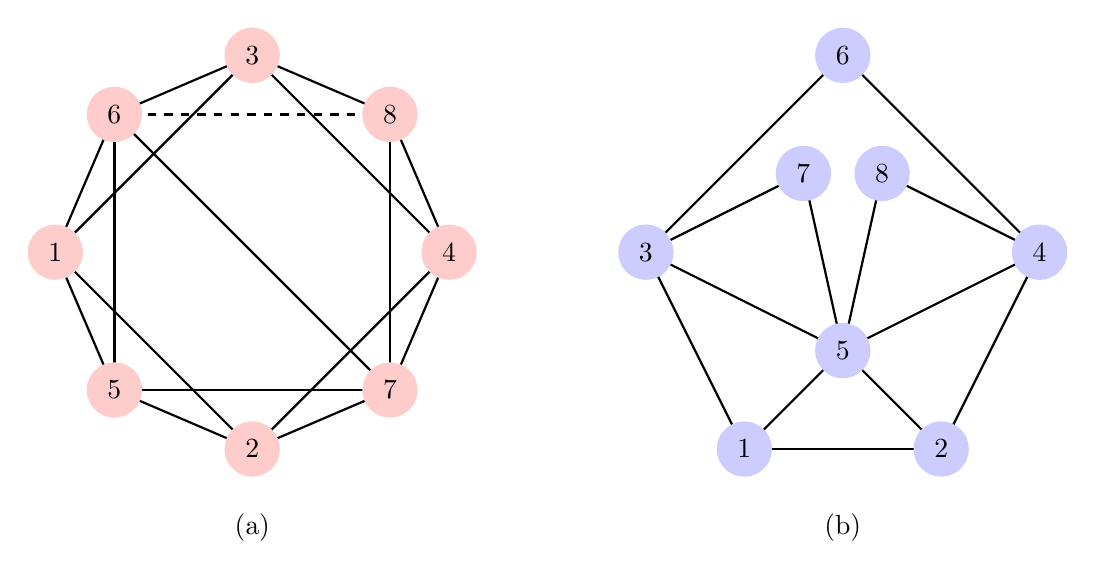
\begin{tikzpicture}[scale=0.5]
\draw[thick] (0,5) -- (5,0);
\draw[thick] (10,5) -- (5,0);
\draw[thick] (5,10) -- (10,5);
\draw[thick] (5,10) -- (0,5);
\draw[thick] (1.5,1.5) -- (1.5,8.5);
\draw[thick, dashed] (1.5,8.5) -- (8.5,8.5);
\draw[thick] (1.5,8.5) -- (8.5,1.5);
\draw[thick] (8.5,8.5) -- (8.5,1.5);
\draw[thick] (8.5,1.5) -- (1.5,1.5);
\draw[thick] (0,5) -- (1.5,1.5);
\draw[thick] (1.5,1.5) -- (5,0);
\draw[thick] (5,0) -- (8.5,1.5);
\draw[thick] (8.5,1.5) -- (10,5);
\draw[thick] (10,5) -- (8.5,8.5);
\draw[thick] (8.5,8.5) -- (5,10);
\draw[thick] (5,10) -- (1.5,8.5);
\draw[thick] (1.5,8.5) -- (0,5);

\draw[thick] (17.5,0) -- (22.5,0);
\draw[thick] (17.5,0) -- (15,5);
\draw[thick] (17.5,0) -- (20,2.5);
\draw[thick] (22.5,0) -- (20,2.5);
\draw[thick] (22.5,0) -- (25,5);
\draw[thick] (25,5) -- (20,2.5);
\draw[thick] (25,5) -- (20,10);
\draw[thick] (25,5) -- (21,7);
\draw[thick] (20,2.5) -- (19,7);
\draw[thick] (20,2.5) -- (15,5);
\draw[thick] (15,5) -- (20,10);
\draw[thick] (20,2.5) -- (21,7);
\draw[thick] (19,7) -- (15,5);

\draw (0,5) node[minimum size=2em,circle,fill=red!20] {$1$};
\draw (5,0) node[minimum size=2em,circle,fill=red!20] {$2$};
\draw (5,10) node[minimum size=2em,circle,fill=red!20] {$3$};
\draw (10,5) node[minimum size=2em,circle,fill=red!20] {$4$};
\draw (1.5,1.5) node[minimum size=2em,circle,fill=red!20] {$5$};
\draw (1.5,8.5) node[minimum size=2em,circle,fill=red!20] {$6$};
\draw (8.5,1.5) node[minimum size=2em,circle,fill=red!20] {$7$};
\draw (8.5,8.5) node[minimum size=2em,circle,fill=red!20] {$8$};
\draw (17.5,0) node[minimum size=2em,circle,fill=blue!20] {$1$};
\draw (22.5,0) node[minimum size=2em,circle,fill=blue!20] {$2$};
\draw (15,5) node[minimum size=2em,circle,fill=blue!20] {$3$};
\draw (25,5) node[minimum size=2em,circle,fill=blue!20] {$4$};
\draw (20,2.5) node[minimum size=2em,circle,fill=blue!20] {$5$};
\draw (20,10) node[minimum size=2em,circle,fill=blue!20] {$6$};
\draw (19,7) node[minimum size=2em,circle,fill=blue!20] {$7$};
\draw (21,7) node[minimum size=2em,circle,fill=blue!20] {$8$};

\draw (5,-2) node {(a)};
\draw (20,-2) node {(b)};
\end{tikzpicture}
\end{center}
\caption[Small-world and scale-free networks]{Network (a) shows a circular small-world model and network (b) shows a scale-free model.}
\label{networks}
\end{figure}

\paragraph{Random graph models.}

The first set of network formation models to be developed are based on the random generation of links between nodes. A random graph is a general term that refers to probability distributions over graphs. Random graphs may be described by a probability distribution, or by a random process which generates them. They are obtained by having an initial set of unconnected nodes and then randomly connecting nodes together by a set of links. The initial research into random graph models was conducted by \citet{ErdosRenyi1959}. The seminal model developed serves as the basis for all subsequent random graph models \citep{Gilbert1959, Bollobas2001}.

A number of properties are derived from the random graph models. An important property is that of a \emph{phase transition}. A phase transition refers to a punctuated change in the state, structure and dynamics of a complex system, that arises from a slight change in a variable that characterises the system as a whole. In the context of an Erd\"{o}s-R\'{e}nyi graph, if the probability of nodes being connected falls below a certain threshold the network will most certainly be \emph{disconnected}, such that there will exist at least one node that is not connected---at least indirectly---to other nodes and thus there cannot exist a strongly connected network. Above the threshold then the network will be strongly connected. The phase transition from a connected network to a disconnected network thus occurs when the probability of nodes being connected falls below a well-defined level.

Although theoretically compelling, many social and economic networks are not formed `randomly'. For example, empirical social networks are much more clustered than those generated by random. Real-world networks are neither completely ordered nor completely random, but rather exhibit important properties of both. Models of small-world networks add `order' to the network by assuming a regular lattice as the starting point.

\paragraph{Small-world networks.}

A small-world network is one whereby nodes are not necessarily neighbours of one another, but most nodes can be reached from every other by a small number of steps. In this form of network, \citet{WattsStrogatz1998}, \citet{Watts1999}, and \citet{NewmanStrogatzWatts2001} generate networks by starting with a symmetric, regular network and randomly rewiring some links between nodes. They found that the random rewiring process leads to an exponential decrease in the average distance between any two nodes whilst maintaining a network that is much more clustered than just randomly wiring the network. Figure~\ref{networks} (a) effectively shows the Watts-Strogatz model of small-world networks. In this example, a regular lattice is generated on a set of eight nodes whereby each node has four links each. Node 6 is rewired to another randomly, which reduces the average path length of the network.

\citet{Kleinberg2000a, Kleinberg2000b} also provides an algorithmic approach to modelling the small-world phenomenon in which he develops a decentralised algorithm to derive the efficient amount of randomness required to generate a small-world network. In the economics literature, \citet{JacksonRogers2005} provide a game theoretic approach to the formation of pairwise stable small-world networks where agents wish to maximise the amount of information they have access to either directly or indirectly given that the information flowing through the network depreciates the longer the geodesic path from one node to another.

\paragraph{Scale-free networks.}

A scale-free network is one in which the number of links that an actor has in the network is unequally distributed such that there exists a minority of actors with many links and a majority of actors with relatively few links. Actors with relatively many links are hubs whose presence reduces the diameter of the network. Research by \citet{Price1976}, \citet{BarabasiAlbert1999}, and \citet{CooperFrieze2003} has shown that networks with power law degree distributions result if nodes form links through the process of \emph{preferential attachment} (i.e., new nodes link to existing nodes with probabilities proportional to the existing nodes' degrees). Power-law distributions have also been shown to result if new nodes copy the links of a randomly identified node \citep{Kleinberg1999, Kumar2000}, or if networks are designed to optimise tolerance \citep{Fabrikant2003}. A variation on preferential attachment where only some nodes are active at any time \citep{Klemm2002a} has been shown to also exhibit small world properties. Some network models that grow over time have been shown to exhibit assortativity and scale-freeness, e.g., \citet{Callaway2001} and \citet{Krapivsky2002}.

Research has shown that many social and economic networks share a scale-free property \citep{Faloutsos1999, DorogovtsevMendes2003, Barabasi2009, Barabasi2012}. Also, biological and mechanical networks also share this structure \citep{Barabasi2011}. Scale-free networks have a number of desirable qualities including robustness to random attacks and small diameters \citep{AlbertJeongBarabasi1999, AlbertJeongBarabasi2000}. As a consequence, scale-free networks are prone to collapse due to targeted attacks and contagious processes.

While the aforementioned models result in some of the empirical regularities of large social networks, none of them are consistent with all of the characteristics above. The closest network formation process to cover all of these properties is indeed from \citet{JacksonRogers2007} whereby agents enter the network and initially form a network randomly, then create other links to nodes based on the initial connections' links. This formation process---a hybrid between random and strategic network formation---provides a structure that is most resembling real social networks. However, it is still questionable as to whether the methods of generating these `social' networks are actually resembling the processes underlying most of the large networks that we actually observe.

For the moment we are only interested in the structure and the methods of forming networks. In Chapter~\ref{ch:relationaltheory} we consider the formation of exchange networks under an algorithmic process. We find that depending on the method of exchange between nodes the overall structure of the network and the average utility of the population changes. The generation of these networks serves as a basis for the algorithmic generation of economic relationships.

\subsection{Economic networks}

There are many studies of markets as networks \citep{RauchCasella2001}. \citet{Uzzi1996} provides one of the most influential investigations regarding the importance of social relationships in the New York City clothing industry. He focussed on the type of relationship between the clothing firms. Specifically, he categorised relationship as ``market'' or ``arm's length'', which included one-time social and economic interactions; and ``special'' or ``close'' interactions, which included many relationships with repeated interactions. Uzzi found that three main aspects were important for these relationships and interactions, these are joint problem-solving; trust; and information transfer. From his analysis, he found that firms with more clustered and intertwined social and economic relationships have a greater probability of survival. To Uzzi, social and economic embeddedness helps firms to survive and thrive. The study also stressed the important interrelatedness of economic and social relationships.

\citet{Weisbuch2000} and \citet{KirmanVriend2001} consider the Marseille Fish Market where market prices are not posted publicly. This allows prices to be maximally flexible: Each producer decides about her own prices; different consumers might be set different prices, and prices can vary over time. Prices are communicated privately and there is no bargaining in this market. A number of outcomes emerge. First, there is widespread loyalty to a single producer, while the minority of consumers purchase from multiple producers. The market promotes trust and reciprocity between consumers and producers. Specifically, consumers follow an adaptive updating rule, with a higher tendency to visit producers who have met their demands in the past. \citet{Vignes1993} and \citet{VignesEtienne2011} assess the network structure and the distribution of price levels throughout the market. The trade pattern that emerges has an interesting feature in that there is persistent price dispersion that fits with the networked structure of the market. The network tended to follow a scale-free structure.

\citet{Granovetter1973} famously considered the labour market a social network of references. As part of his PhD thesis, he investigated how people within a certain professional socio-economic class typically found information regarding new job opportunities. He identified that people tended to obtain the most relevant information about job availability from contacts in their social neighbourhood. Less intuitively, he found that the best information often came from acquaintances as opposed to close friends or family. Granovetter claimed that every person who forms social relationships holds a mixture of both \emph{strong} and \emph{weak} ties; where strong ties pertained to close friends and family members, and weak ties pertained to acquaintances. According to Granovetter, the labour market operates as a social network where information regarding job opportunities are disseminated through the network. Weak ties, as opposed to strong ties, held less redundant and therefore more diverse information which an individual could exploit when attaining a job. Much in the same vein as Granovetter, \citet[p.~333]{Jackson2008} suggests that social networks of a firms' existing employees can also provide a good resource for searching for suitable employees, `` [a] firm may simply want to hire people similar to the employees it already has. Given the homophily in many social networks, a firm can take advantage of its existing workforce to find other people with similar characteristics.'' The outcome of the assessment is that the labour market that exists is more intricate than one characterised by traditional microeconomic analysis of labour economics.

The theory of weak and strong ties has been the cornerstone of much of economic sociology since Granovetter's initial findings. The weakest, and therefore most valuable in terms of information, relations are \emph{bridge} relations. These were discussed in depth by \citet{Burt1992}, who suggested that individuals could exploit these bridge relationships through the attainment of new and diverse sets of information \citep{Burt2004}. As such, there exist positions of power within social networks and networked markets where some positions are more influential than other positions.

Exchange theory is concerned with how the structure of relationships among agents affects exchange between them \citep{CookWhitmeyer1992}. These exchanges could include economic interactions, trading of favours, communication of information, or other social interactions. Typically this research is based on dyadic interactions, but since the work of Robert \citet{Emerson1962, Emerson1972a, Emerson1972b, Emerson1976} networks have played an increasingly important role in exchange theory. In his work, Emerson considered network interactions to explain power and dependencies when considering an exchange. This theory of networks played a role in Emerson's work because all economic exchange depended on the availability of outside options; therefore assuming a relatively competitive market in which economic relations could be made and severed without any friction. Under such a perspective, an economic interaction cannot be viewed without the context of the complete network of all potential interactions and relationships. Again, much like Burt, network positions matter and asymmetries of power tend to be expected.

\subsubsection{Models of economic networks}

Emerson's work combined with the mathematical research of matching in bipartite graphs \citep{Hall1935} provided the basis for more research in bilateral trading models \citep{Corominas-Bosch1999, Corominas-Bosch2004}. Much like the implicit assumption of general equilibrium models, these models assume a dichotomy between the demand and supply within an economy. Therefore, all networks that emerge are simply between a set of nodes who produce the supply of the economy and a set of nodes who demand the produced goods. \citet{Blume2009} provide a convincing model of economic exchange on networks. They also dichotomise the forces of demand and supply by introducing a set of `consumers' and a set of `producers' whereby a consumer can only engage in an economic exchange with a producer. Each economic exchange is represented as a link. As a consequence, a bipartite network is formed whereby economic exchange occurs across the links between consumers and producers. The structure of their model follows that of \citet{KrantonMinehart2001} whereby, again, the forces of demand and supply are partitioned therefore forming two disjoint sets of consumers and producers. This bipartite set-up is also taken by \citet[Chapter~10]{Jackson2008}. Easley and Kleinberg find that this networked structure provides some nice properties, being able to show that society's welfare is maximised when prices develop to guide consumers to producers. Moreover, they find that, along with \citet{Kakade2004a, Kakade2004b}, a network provides a good basis for price dispersion as was seen in the Marseille fish market case.

\begin{figure}[t]
\begin{center}
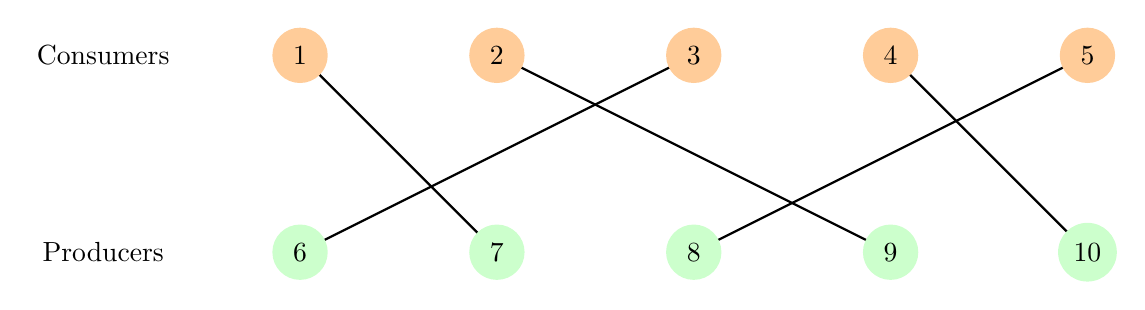
\begin{tikzpicture}[scale=0.5]
\draw[thick] (5,0) -- (15,5);
\draw[thick] (10,0) -- (5,5);
\draw[thick] (20,0) -- (10,5);
\draw[thick] (15,0) -- (25,5);
\draw[thick] (25,0) -- (20,5);

\draw (5,0) node[minimum size=2em,circle,fill=green!20] {$6$};
\draw (5,5) node[minimum size=2em,circle,fill=orange!40] {$1$};

\draw (10,0) node[minimum size=2em,circle,fill=green!20] {$7$};
\draw (10,5) node[minimum size=2em,circle,fill=orange!40] {$2$};

\draw (15,0) node[minimum size=2em,circle,fill=green!20] {$8$};
\draw (15,5) node[minimum size=2em,circle,fill=orange!40] {$3$};

\draw (20,0) node[minimum size=2em,circle,fill=green!20] {$9$};
\draw (20,5) node[minimum size=2em,circle,fill=orange!40] {$4$};

\draw (25,0) node[minimum size=2em,circle,fill=green!20] {$10$};
\draw (25,5) node[minimum size=2em,circle,fill=orange!40] {$5$};

\draw (0,0) node {Producers};
\draw (0,5) node {Consumers};
\end{tikzpicture}
\end{center}
\caption{A matching market of consumers and producers}
\label{fig:bipartiteexchange}
\end{figure}

This bipartite representation of a market, known as a ``matching market'', can be seen in Figure~\ref{fig:bipartiteexchange}. This notion of a matching market is further extended by \citet{EasleyKleinberg2010} to include `traders' as intermediaries between consumers and producers. From this they informally define a notion of competition in a networked economy, suggesting that traders have an opportunity to monopolise flows of economic exchange between producers and consumers. The notion regarding the monopolisation of trade is extended and considered in detail in Chapters~\ref{ch:criticalnodes} and~\ref{ch:blocks} where we discuss measurements of brokerage in networked economies.

The reason why networks follow a bipartite structure is due to the way in which economic agents are characterised within the traditional perspective, and specifically the strict dichotomy between demand and supply~\footnote{When generating economic networks in Chapter~\ref{ch:relationaltheory} we do not assume the existence of a strict dichotomy between consumption and production and, as a direct consequence, a bipartite network does not typically emerge. Instead, when generating the exchange networks we arrive at properties that are more closely related to the typical structure of social networks as noted by the characteristics above.}. Within this monograph, we note that economic agents are boundedly rational and exist within a network of social and economic relations that are influenced by systems of governance. However, the economic agent is further defined such that each individual is endowed with the powers of both production and consumption; that the forces of demand and supply are contained in all individual economic agents.

\section{Monograph structure}

This monograph is partitioned into three interlinked parts, each of which addresses the ultimate goal of developing a theory of the entrepreneur and entrepreneurial activity within a relational perspective of socio-economic activity. The first two parts are primarily focussed on theory, occasionally using empirical examples to illustrate and test models and measures. The final part is more focussed on explaining entrepreneurial activities within real-world case studies. Part~\ref{part:generalTheoryEntrepreneurship} consists of three chapters that provide a theoretical foundation to the relational perspective and an introduction to the entrepreneur. Much effort is spent developing the relational perspective framework, which is done from an evolutionary basis of the social actor that in turn represents an economic agent. Within this framework we are able to provide a holistic definition of the entrepreneur, linking the notion appropriately to the social division of labour and the networked structure that economic interaction produces. Of specific interest are the unique positions within the network that the entrepreneurial agent operates, and can be a source of their economic utility.

Part~\ref{part:entrepreneurshipPlatonianEconomy} consists of two chapters that elaborate on the interaction between entrepreneurship and the network interaction infrastructure. We investigate the establishment of uncontested middleman positions and the formation of blocks in relational economies. In elaborating on these concepts we develop formal models and measures to use on network-based data sets. These models and measures are then tested against the empirical data.

Part~\ref{part:entrepreneurshipPlatformEconomy}, the final Part of the monograph, also consists of two chapters that introduce an elaborate example of power within a more developed economy. This economic space is representative of a more layered economy within which there exist firms and directors that operate in multiple complementary industries. We analyse the directorial network and interlock formation in New York City from in the early Twentieth century as an entrepreneurial process. Indeed, these chapters investigate the establishment of power in New York City through network entrepreneurship and provide measures and models to investigate the centralisation of economic influence and use this to challenge claims regarding the history of the so-called \emph{Empire State} and the role of J.P. Morgan.